\documentclass{article}
\setlength{\parskip}{0pt} % esp. entre parrafos
\setlength{\parindent}{3pt} % esp. al inicio de un parrafo
\usepackage{amsmath} % mates
\usepackage{listings}
\usepackage[sort&compress,numbers]{natbib} % referencias
\usepackage{url} % que las URLs se vean lindos
\usepackage[top=15mm,left=20mm,right=20mm,bottom=25mm]{geometry} % \textbf{\textbf{}}margenes
\usepackage{hyperref} % ligas de URLs
\usepackage{graphicx} % poner figuras
\usepackage{subfigure}
\usepackage[spanish]{babel} % otros idiomas
\hypersetup{
    colorlinks=true,
    linkcolor=blue,
    filecolor=blue,      
    urlcolor=blue,
    citecolor=black,
}

\title{TAREA \# 10 \\ Algoritmo genético} %titulo
\author{Natalia Berenice P\'{e}rez L\'{o}pez} % author
\date{\today}

\begin{document} % inicia contenido

\maketitle % cabecera

\section{Objetivo}
El objetivo de esta práctica es generar tres instancias con tres distintas reglas (nueve en total):
\bigskip

Regla 1: el peso y el valor de cada objeto se generan independientemente con una distribución uniforme.
\smallskip

Regla 2: el valor de cada objeto se genera independientemente con una distribución exponencial y su peso es inversamente correlacionado con el valor.
\smallskip

Regla 3: el peso de cada objeto se generan independientemente con una distribución normal y su valor es (positivamente) correlacionado con el cuadrado del peso, con un ruido normalmente distribuido de baja magnitud.
\smallskip

Determinar para cada uno de los tres casos si variar la probabilidad de mutación, la cantidad de cruzamientos y el tamaño de la población (dos o tres niveles basta) tienen un efecto (solo o en combinación) estadísticamente significativo (usando por lo menos tres réplicas por instancia) en la calidad de resultado, manteniendo el tiempo de ejecución fijo.

\section{Desarrollo} % seccion y etiqueta
Para generar los códigos de esta práctica se realizaron algunas ideas y pruebas iniciales, las cuales se encuentran en \href{https://github.com/nataliaperez0/Simulation/tree/main/Tarea10}{mi repositorio}  en GitHub. Se inició tomando como base el código revisado en clase para ejecutar una cantidad predeterminada de generaciones, primero mutando, luego reproduciendo, y al final cortando el tamaño de la población a la misma que estuvo al inicio de la iteración, dando preferencia a las soluciones factibles \citep{1}. Se realizaron tres códigos diferentes para cada regla mencionada en el objetivo de la práctica, y para cada regla se realizaron tres códigos más para variar la probabilidad de mutación, la cantidad de cruzamientos y el tamaño de la población en cada código respectivamente. Para el código que mantiene el tiempo de ejecución fijo me apoyé en el repositorio de mi compañero Eduardo Navarro \citep{2}.
\bigskip

A continuación se muestran los códigos para cada regla:
\bigskip

\textbf{REGLA 1:} el peso y el valor de cada objeto se generan independientemente con una distribución uniforme.

\definecolor{verde}{rgb}{0,0.56,0.22}
\definecolor{codegray}{rgb}{0.5,0.5,0.5}
\definecolor{codegreen}{rgb}{0,0.56,0.22}
\definecolor{backcolour}{rgb}{0.95,0.95,0.92}
\definecolor{azul}{rgb}{0,0,1}

\lstdefinestyle{mystyle}{
    backgroundcolor=\color{backcolour},   
    commentstyle=\color{verde},
    keywordstyle=\color{azul},
    numberstyle=\tiny\color{codegray},
    stringstyle=\color{codegreen},
    basicstyle=\ttfamily\footnotesize,
    breakatwhitespace=false,         
    breaklines=true,                 
    captionpos=b,                    
    keepspaces=true,                 
    numbers=left,                    
    numbersep=5pt,                  
    showspaces=false,                
    showstringspaces=false,
    showtabs=false,                  
    tabsize=2
}

\lstset{style=mystyle}
\begin{lstlisting}[language=R, caption= Código para cumplir la regla 1.]
#pesos independientes con distribucion uniforme
generador.pesos <- function(cuantos, min, max) {
  return(sort(round((runif(cuantos)) * (max - min) + min)))
}
#valores independientes con distribucion uniforme
generador.valores <- function(cuantos, min, max) {
  return(round((runif(cuantos)) * (max - min) + min))
}
\end{lstlisting}

\textbf{REGLA 2:} el valor de cada objeto se genera independientemente con una distribución exponencial y su peso es inversamente correlacionado con el valor.

\lstset{style=mystyle}
\begin{lstlisting}[language=R, caption= Código para cumplir la regla 2.]
#valores independientes con distribucion exponencial
generador.valores <- function(cuantos, min, max) {
  return(round(normalizar(rexp(cuantos)) * (max - min) + min))
}

#pesos inversamente correlacionados con el valor
generador.pesos <- function(valores, min, max) {
  n <- length(valores)
  pesos <- double()
  for (i in 1:n) {
    media <- valores[i]
    desv <- runif(1, max=0.1)
    pesos <- c(pesos, rnorm(1, (1/media), desv))
  }
  pesos <- normalizar(pesos) * (max - min) + min
  return(pesos)
}
\end{lstlisting}

\textbf{REGLA 3:} el peso de cada objeto se genera independientemente con una distribución normal y su valor es (positivamente) correlacionado con el cuadrado del peso, con un ruido normalmente distribuido de baja magnitud.

\lstset{style=mystyle}
\begin{lstlisting}[language=R, caption= Código para cumplir la regla 3.]
#pesos independientes con distribucion normal
generador.pesos <- function(cuantos, min, max) {
  return(sort(round(normalizar(rnorm(cuantos)) * (max - min) + min)))
}
#valores correlacionados con el cuadrado del peso con ruido normalmente distribuido de baja magnitud
generador.valores <- function(pesos, min, max) {
  n <- length(pesos)
  valores <- double()
  for (i in 1:n) {
    media <- pesos[i]
    desv <- runif(1)
    ruido <- rnorm(1, sd=.1)
    valores <- c(valores, rnorm(1, media^2, desv) + ruido)
  }
  valores <- normalizar(valores) * (max - min) + min
  return(valores)
}
\end{lstlisting}

A continuación se muestran los tres códigos que se ejecutaron con cada regla:
\bigskip

\textbf{Código 1:} variar la probabilidad de mutación en tres niveles (0.1, 0.3 y 0.6) y hacer tres réplicas.

\lstset{style=mystyle}
\begin{lstlisting}[language=R, caption= Fragemento del código para variar la probabilidad de mutación en tres niveles.]
df = data.frame()
mut = c(0.1, 0.3, 0.6) #variar probabilidad de mutacion
rep <- 10 #cantidad de cruzamientos

for (pm in mut){
  for (replica in 1:3){
    n <- 60 #cuantos objetos
    pesos <- generador.pesos(n, 15, 80)
    valores <- generador.valores(pesos, 10, 500)
    capacidad <- round(sum(pesos) * 0.65)
    optimo <- knapsack(capacidad, pesos, valores)
    init <- 30  #cuantas soluciones
    p <- poblacion.inicial(n, init)
    tam <- dim(p)[1]
    assert(tam == init)
    mejores <- double()
    
    tiempo = 10 #segundos
    start = Sys.time()
    
    while(TRUE) {
      elapsed = as.numeric(difftime(Sys.time(), start, units = 'secs'))
      remaining = tiempo - round(elapsed) 
      Sys.sleep(0.1)
      print(remaining)
      
      p$obj <- NULL
      p$fact <- NULL
      for (i in 1:tam) { # cada objeto puede mutarse con probabilidad pm
        if (runif(1) < pm) {
          p <- rbind(p, mutacion(p[i,], n))
        }
      }
      for (i in 1:rep) { # una cantidad fija de reproducciones
        padres <- sample(1:tam, 2, replace=FALSE)
        hijos <- reproduccion(p[padres[1],], p[padres[2],], n)
        p <- rbind(p, hijos[1:n]) # primer hijo
        p <- rbind(p, hijos[(n+1):(2*n)]) # segundo hijo
      }
      tam <- dim(p)[1]
      obj <- double()
      fact <- integer()
      for (i in 1:tam) {
        obj <- c(obj, objetivo(p[i,], valores))
        fact <- c(fact, factible(p[i,], pesos, capacidad))
      }
      p <- cbind(p, obj)
      p <- cbind(p, fact)
      mantener <- order(-p[, (n + 2)], -p[, (n + 1)])[1:init]
      p <- p[mantener,]
      tam <- dim(p)[1]
      assert(tam == init)
      factibles <- p[p$fact == TRUE,]
      mejor <- max(factibles$obj)
      mejores <- c(mejores, mejor)
      
      print(paste(mejor, (optimo - mejor) / optimo))
      opt <- ((optimo - mejor) / optimo)*100
      segundos <-round(elapsed)
      
      if (remaining <= 0) break
      
      resultado = c(pm, replica, segundos, mejor, opt, optimo)
      df = rbind(df, resultado)
      names(df) = c("Mutacion", "Replica", "Segundo", "Mejor", "Gap", "Optimo")
    }
  }
}
\end{lstlisting}

En el código anterior se muestra el ciclo \texttt{While} para mantener un tiempo de ejecución fijo de $10$ segundos en lugar de hacer iteraciones.
\bigskip

\textbf{Código 2:} variar la cantidad de cruzamientos en tres niveles (10, 15 y 20) y hacer tres réplicas.

\lstset{style=mystyle}
\begin{lstlisting}[language=R, caption= Fragemento del código para variar la cantidad de cruzamientos en tres niveles.]
df = data.frame()
cruz = c(10, 15, 20) #variar la cantidad de cruzamientos
pm = 0.1 #probabilidad de mutacion

for (rep in cruz){
  for (replica in 1:3){
    n <- 60 #cuantos objetos
    pesos <- generador.pesos(n, 15, 80)
    valores <- generador.valores(pesos, 10, 500)
    capacidad <- round(sum(pesos) * 0.65)
    optimo <- knapsack(capacidad, pesos, valores)
    init <- 30  #cuantas soluciones
    p <- poblacion.inicial(n, init)
    tam <- dim(p)[1]
    assert(tam == init)
    mejores <- double()
    
    tiempo = 10 #segundos
    start = Sys.time()
    
    while(TRUE) {
      elapsed = as.numeric(difftime(Sys.time(), start, units = 'secs'))
      remaining = tiempo - round(elapsed) 
      Sys.sleep(0.1)
      print(remaining)
\end{lstlisting}

\textbf{Código 3:} variar el tamaño de la población en tres niveles (25, 35 y 45) y hacer tres réplicas.

\lstset{style=mystyle}
\begin{lstlisting}[language=R, caption= Fragemento del código para variar el tamaño de la población en tres niveles.]
df = data.frame()
pm = 0.1 #probabilidad de mutacion
rep <- 15 #cantidad de cruzamientos
solu = c(25, 35, 45) #cuantas soluciones

for (init in solu){
  for (replica in 1:3){
    n <- 60 #cuantos objetos
    pesos <- generador.pesos(n, 15, 80)
    valores <- generador.valores(pesos, 10, 500)
    capacidad <- round(sum(pesos) * 0.65)
    optimo <- knapsack(capacidad, pesos, valores)
    p <- poblacion.inicial(n, init)
    tam <- dim(p)[1]
    assert(tam == init)
    mejores <- double()
    
    tiempo = 10 #segundos
    start = Sys.time()
    
    while(TRUE) {
      elapsed = as.numeric(difftime(Sys.time(), start, units = 'secs'))
      remaining = tiempo - round(elapsed) 
      Sys.sleep(0.1)
      print(remaining)
\end{lstlisting}

En la figura \ref{f1} se muestran los diagramas caja-bigote para cada probabilidad de mutación del \texttt{código 1} de la \texttt{regla 1}.

En la figura \ref{f2} se muestran los diagramas caja-bigote para cada cantidad de cruzamientos del \texttt{código 2} de la \texttt{regla 1}.

En la figura \ref{f3} se muestran los diagramas caja-bigote para cada tamaño de población del \texttt{código 3} de la \texttt{regla 1}.
\bigskip

En la figura \ref{f4} se muestran los diagramas caja-bigote para cada probabilidad de mutación del \texttt{código 1} de la \texttt{regla 2}.

En la figura \ref{f5} se muestran los diagramas caja-bigote para cada cantidad de cruzamientos del \texttt{código 2} de la \texttt{regla 2}.

En la figura \ref{f6} se muestran los diagramas caja-bigote para cada tamaño de población del \texttt{código 3} de la \texttt{regla 2}.
\bigskip

En la figura \ref{f7} se muestran los diagramas caja-bigote para cada probabilidad de mutación del \texttt{código 1} de la \texttt{regla 3}.

En la figura \ref{f8} se muestran los diagramas caja-bigote para cada cantidad de cruzamientos del \texttt{código 2} de la \texttt{regla 3}.

En la figura \ref{f9} se muestran los diagramas caja-bigote para cada tamaño de población del \texttt{código 3} de la \texttt{regla 3}.
\bigskip

Para analizar mejor los resultados de los diagramas caja-bigote se realizaron pruebas estadísticas, las cuales se muestran después de cada figura.

\newpage
\begin{figure}[h!]
\centering
\subfigure[Probabilidad de mutación = 0.1]{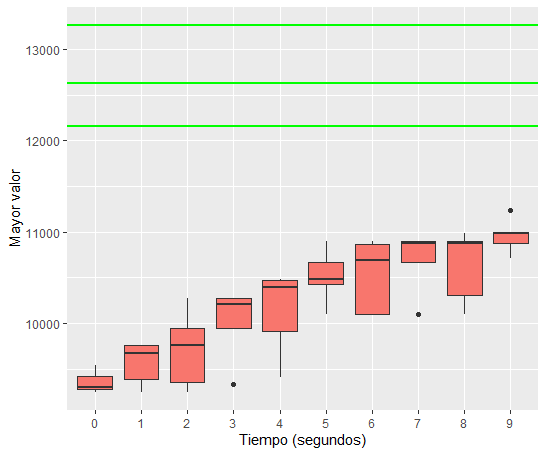
\includegraphics[width=87mm]{FiguraR1C1P0.1.png}}
\subfigure[Probabilidad de mutación = 0.3]{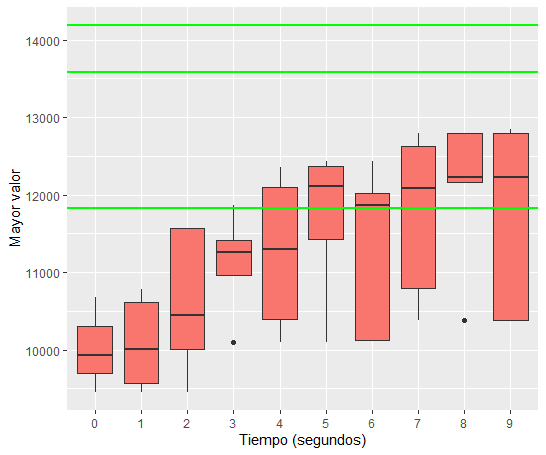
\includegraphics[width=87mm]{FiguraR1C1P0.3.png}}
\subfigure[Probabilidad de mutación = 0.6]{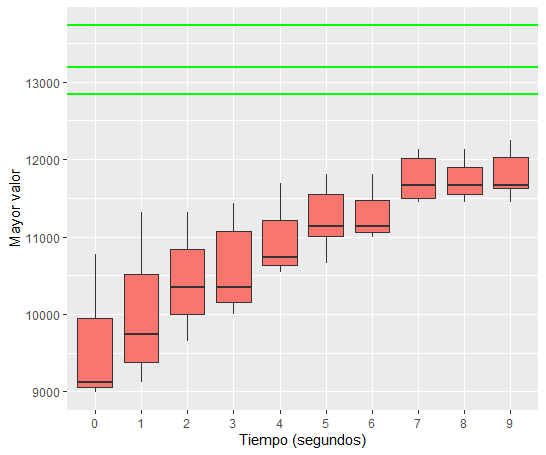
\includegraphics[width=87mm]{FiguraR1C1P0.6.png}}
\caption{Mayor valor para cada tiempo de acuerdo a cada probabilidad de mutación para el código 1 de la regla 1.} 
\label{f1}
\end{figure}

\begin{table}[h!]
\centering
\caption{Resultados de la prueba estadística.}
\smallskip

\begin{tabular}{ |p{4cm}|p{8cm}|}
 \hline
 Outliers & $0$ \\
 \hline
 Normalidad por grupo & $0.1$: $p$ = $0.00348$ / $0.3$: $p$ = $0.00139$ / $0.6$: $p$ = $0.00440$ \\
 \hline
 Kruskal Wallis & $p$ = $8.095\times 10^{-6}$ \\
 \hline
\end{tabular}
\label{Cuadro1}
\end{table}

\begin{table}[h!]
\centering
\caption{Resultados al aplicar la prueba \texttt{Wilcoxon}.}
\smallskip

\begin{tabular}{|p{1.7cm}|p{1.7cm}|p{1.7cm}|}
 \hline
Valor de $p$ & $0.1$ & $0.3$ \\
 \hline
 $0.3$ & $0.00015$ & -   \\
 \hline
 $0.6$ & $0.00004$ & $0.29082$  \\
 \hline
\end{tabular}
\label{Cuadro2}
\end{table}

Hipótesis nula : Las medias son iguales en todos los grupos. Se rechaza esta hipótesis, si hay diferencias significativas de las medias.

\newpage
\begin{figure}[h!]
\centering
\subfigure[Cruzamientos = 10]{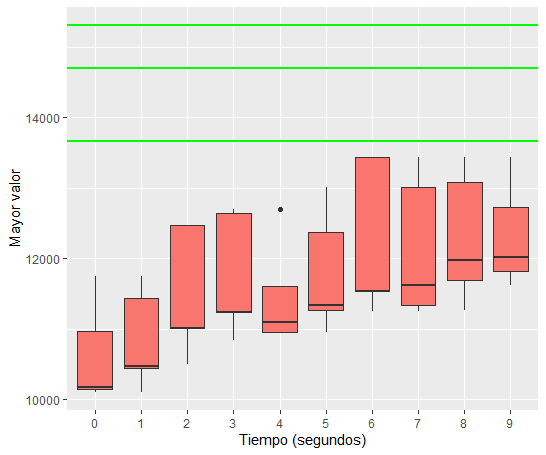
\includegraphics[width=87mm]{FiguraR1C2R10.png}}
\subfigure[Cruzamientos = 15]{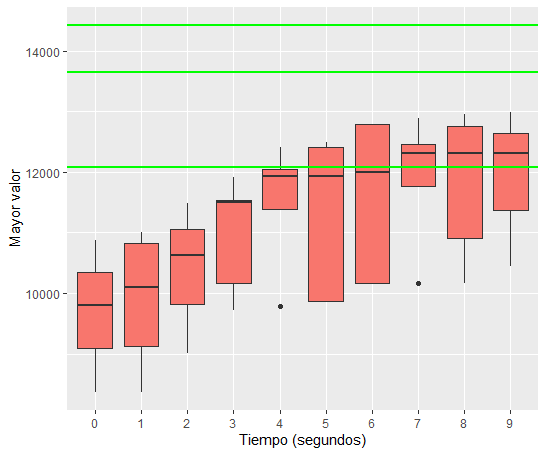
\includegraphics[width=87mm]{FiguraR1C2R15.png}}
\subfigure[Cruzamientos = 20]{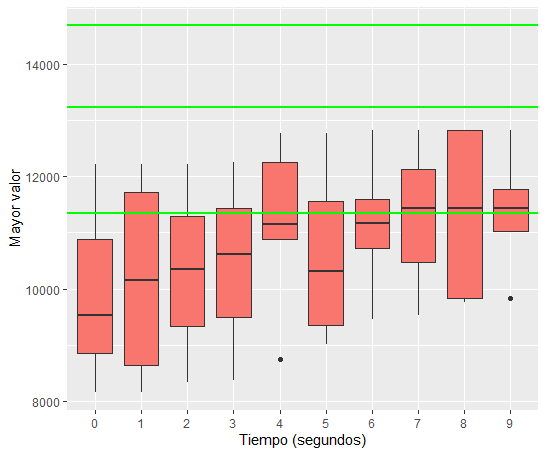
\includegraphics[width=87mm]{FiguraR1C2R20.png}}
\caption{Mayor valor para cada tiempo de acuerdo a cada cantidad de cruzamientos para el código 2 de la regla 1.} 
\label{f2}
\end{figure}

\begin{table}[h!]
\centering
\caption{Resultados de la prueba estadística.}
\smallskip

\begin{tabular}{ |p{4cm}|p{8cm}|}
 \hline
 Outliers & $0$ \\
 \hline
 Normalidad por grupo & $10$: $p$ = $0.00571$ / $15$: $p$ = $0.01540$ / $20$: $p$ = $0.00831$ \\
 \hline
 Kruskal Wallis & $p$ = $0.01654$ \\
 \hline
\end{tabular}
\label{Cuadro3}
\end{table}

\begin{table}[h!]
\centering
\caption{Resultados al aplicar la prueba \texttt{Wilcoxon}.}
\smallskip

\begin{tabular}{|p{1.7cm}|p{1.7cm}|p{1.7cm}|}
 \hline
Valor de $p$ & $10$ & $15$ \\
 \hline
 $15$ & $0.091$ & -   \\
 \hline
 $20$ & $0.026$ & $0.250$  \\
 \hline
\end{tabular}
\label{Cuadro4}
\end{table}

Hipótesis nula : Las medias son iguales en todos los grupos. Se rechaza esta hipótesis, si hay diferencias significativas de las medias.

\newpage
\begin{figure}[h!]
\centering
\subfigure[Población = 25]{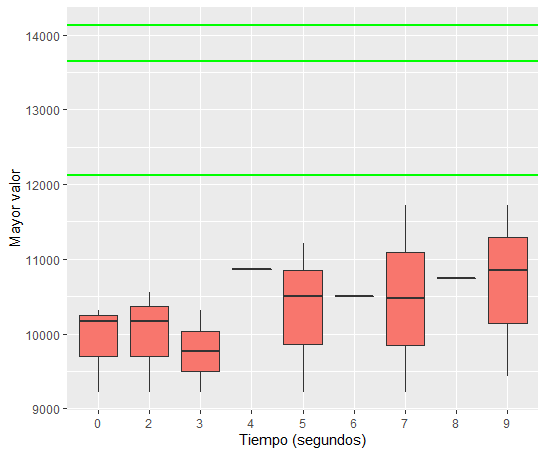
\includegraphics[width=87mm]{FiguraR1C3S25.png}}
\subfigure[Población = 35]{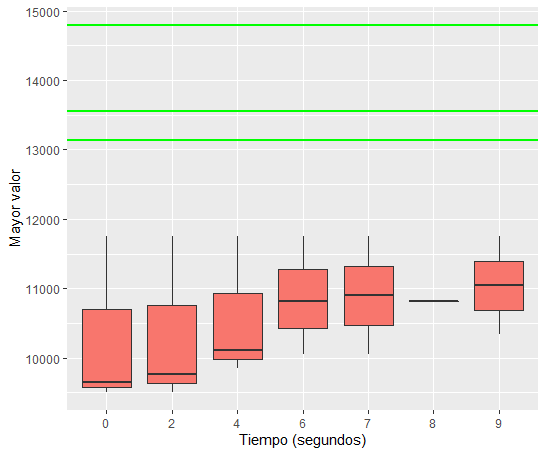
\includegraphics[width=87mm]{FiguraR1C3S35.png}}
\subfigure[Población = 45]{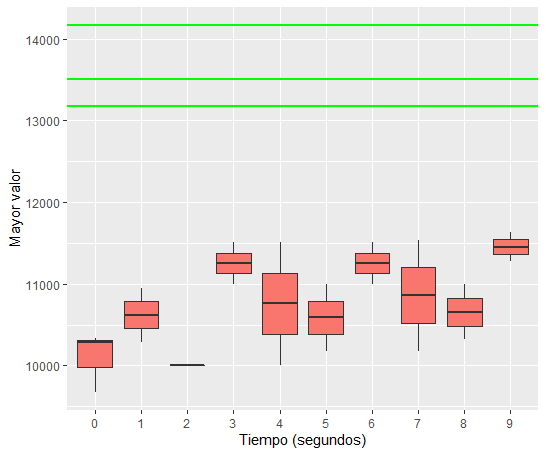
\includegraphics[width=87mm]{FiguraR1C3S45.png}}
\caption{Mayor valor para cada tiempo de acuerdo a cada tamaño de población para el código 3 de la regla 1.} 
\label{f3}
\end{figure}

\begin{table}[h!]
\centering
\caption{Resultados de la prueba estadística.}
\smallskip

\begin{tabular}{ |p{4cm}|p{8cm}|}
 \hline
 Outliers & $0$ \\
 \hline
 Normalidad por grupo & $25$: $p$ = $0.0603$ / $35$: $p$ = $0.0047$ / $45$: $p$ = $0.0494$ \\
 \hline
 Kruskal Wallis & $p$ = $0.2028$ \\
 \hline
\end{tabular}
\label{Cuadro5}
\end{table}

\begin{table}[h!]
\centering
\caption{Resultados al aplicar la prueba \texttt{Wilcoxon}.}
\smallskip

\begin{tabular}{|p{1.7cm}|p{1.7cm}|p{1.7cm}|}
 \hline
Valor de $p$ & $25$ & $35$ \\
 \hline
 $35$ & $0.45$ & -   \\
 \hline
 $40$ & $0.25$ & $0.73$  \\
 \hline
\end{tabular}
\label{Cuadro6}
\end{table}

Hipótesis nula : Las medias son iguales en todos los grupos. Se acepta esta hipótesis.

\newpage
\begin{figure}[h!]
\centering
\subfigure[Probabilidad de mutación = 0.1]{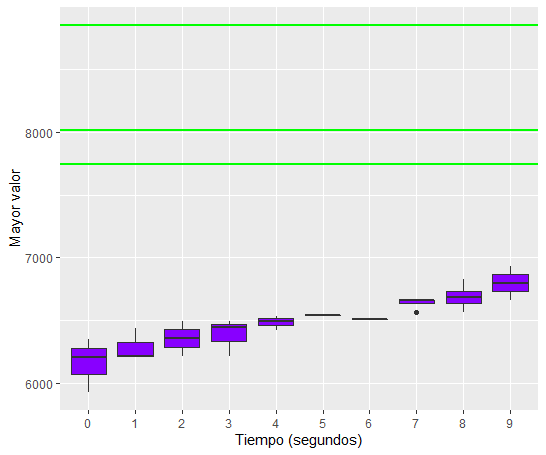
\includegraphics[width=87mm]{FiguraR2C1P0.1.png}}
\subfigure[Probabilidad de mutación = 0.3]{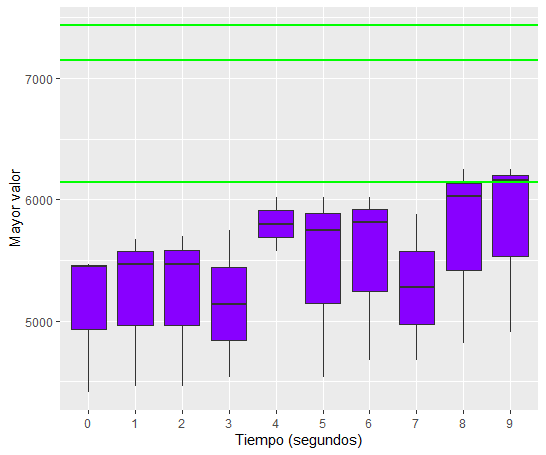
\includegraphics[width=87mm]{FiguraR2C1P0.3.png}}
\subfigure[Probabilidad de mutación = 0.6]{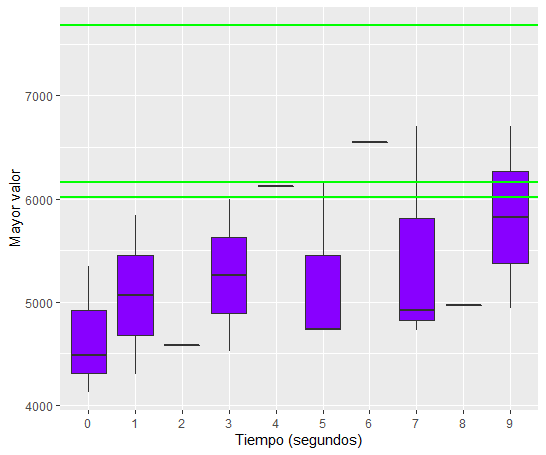
\includegraphics[width=87mm]{FiguraR2C1P0.6.png}}
\caption{Mayor valor para cada tiempo de acuerdo a cada probabilidad de mutación para el código 1 de la regla 2.} 
\label{f4}
\end{figure}

\begin{table}[h!]
\centering
\caption{Resultados de la prueba estadística.}
\smallskip

\begin{tabular}{ |p{4cm}|p{8cm}|}
 \hline
 Outliers & $1$ \\
 \hline
 Normalidad por grupo & $0.1$: $p$ = $0.295$ / $0.3$: $p$ = $0.006$ / $0.6$: $p$ = $0.039$ \\
 \hline
 Kruskal Wallis & $p$ = $7.966\times 10^{-9}$ \\
 \hline
\end{tabular}
\label{Cuadro7}
\end{table}

\begin{table}[h!]
\centering
\caption{Resultados al aplicar la prueba \texttt{Wilcoxon}.}
\smallskip

\begin{tabular}{|p{1.7cm}|p{1.7cm}|p{1.7cm}|}
 \hline
Valor de $p$ & $0.1$ & $0.3$ \\
 \hline
 $0.3$ & $5.7\times 10^{-9}$ & -   \\
 \hline
 $0.6$ & $6.6\times 10^{-5}$ & $0.67$  \\
 \hline
\end{tabular}
\label{Cuadro8}
\end{table}

Hipótesis nula : Las medias son iguales en todos los grupos. Se rechaza esta hipótesis, si hay diferencias significativas de las medias.

\newpage
\begin{figure}[h!]
\centering
\subfigure[Cruzamientos = 10]{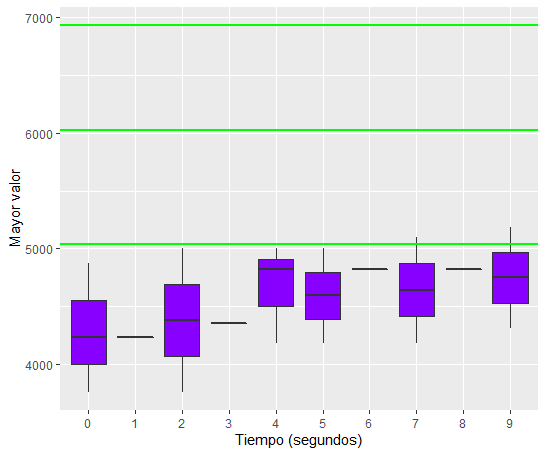
\includegraphics[width=87mm]{FiguraR2C2R10.png}}
\subfigure[Cruzamientos = 15]{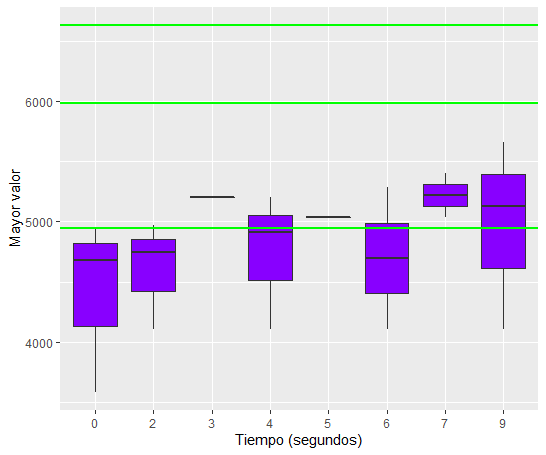
\includegraphics[width=87mm]{FiguraR2C2R15.png}}
\subfigure[Cruzamientos = 20]{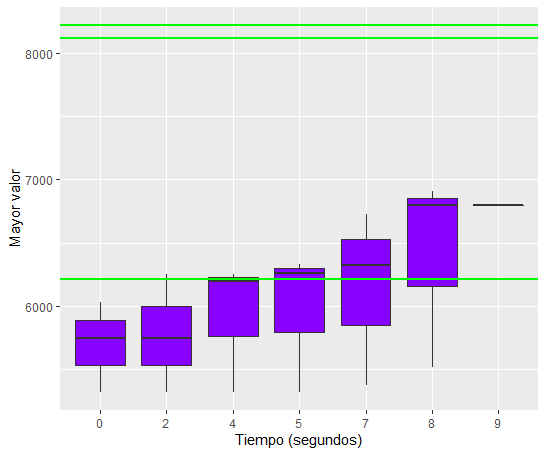
\includegraphics[width=87mm]{FiguraR2C2R20.png}}
\caption{Mayor valor para cada tiempo de acuerdo a cada cantidad de cruzamientos para el código 2 de la regla 2.} 
\label{f5}
\end{figure}

\begin{table}[h!]
\centering
\caption{Resultados de la prueba estadística.}
\smallskip

\begin{tabular}{ |p{4cm}|p{8cm}|}
 \hline
 Outliers & $0$ \\
 \hline
 Normalidad por grupo & $10$: $p$ = $0.054$ / $15$: $p$ = $0.113$ / $20$: $p$ = $0.042$ \\
 \hline
 Kruskal Wallis & $p$ = $2.11\times 10^{-8}$ \\
 \hline
\end{tabular}
\label{Cuadro9}
\end{table}

\begin{table}[h!]
\centering
\caption{Resultados al aplicar la prueba \texttt{Wilcoxon}.}
\smallskip

\begin{tabular}{|p{1.7cm}|p{1.7cm}|p{1.7cm}|}
 \hline
Valor de $p$ & $10$ & $15$ \\
 \hline
 $15$ & $0.19$ & -   \\
 \hline
 $20$ & $6.4\times 10^{-7}$ & $2.4\times 10^{-6}$  \\
 \hline
\end{tabular}
\label{Cuadro10}
\end{table}

Hipótesis nula : Las medias son iguales en todos los grupos. Se rechaza esta hipótesis, si hay diferencias significativas de las medias.

\newpage
\begin{figure}[h!]
\centering
\subfigure[Población = 25]{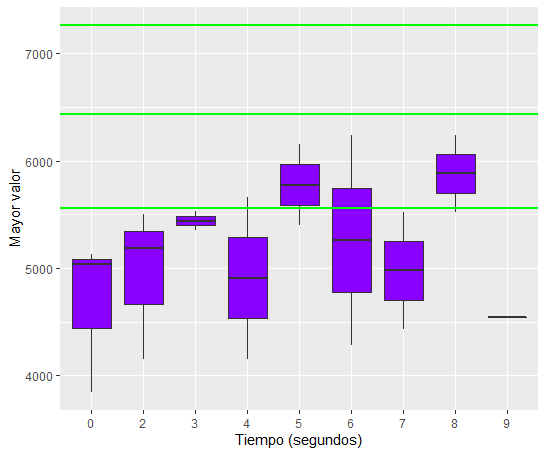
\includegraphics[width=87mm]{FiguraR2C3S25.png}}
\subfigure[Población = 35]{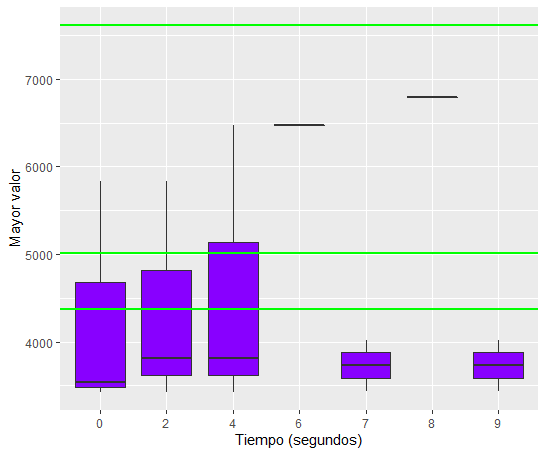
\includegraphics[width=87mm]{FiguraR2C3S35.png}}
\subfigure[Población = 45]{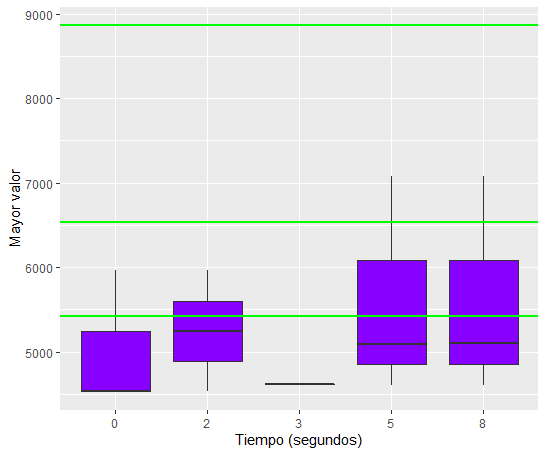
\includegraphics[width=87mm]{FiguraR2C3S45.png}}
\caption{Mayor valor para cada tiempo de acuerdo a cada tamaño de población para el código 3 de la regla 2.} 
\label{f6}
\end{figure}

\begin{table}[h!]
\centering
\caption{Resultados de la prueba estadística.}
\smallskip

\begin{tabular}{ |p{4cm}|p{8cm}|}
 \hline
 Outliers & $0$ \\
 \hline
 Normalidad por grupo & $25$: $p$ = $0.210$ / $35$: $p$ = $0.001$ / $45$: $p$ = $0.005$ \\
 \hline
 Kruskal Wallis & $p$ = $0.07854$ \\
 \hline
\end{tabular}
\label{Cuadro11}
\end{table}

\begin{table}[h!]
\centering
\caption{Resultados al aplicar la prueba \texttt{Wilcoxon}.}
\smallskip

\begin{tabular}{|p{1.7cm}|p{1.7cm}|p{1.7cm}|}
 \hline
Valor de $p$ & $25$ & $35$ \\
 \hline
 $35$ & $0.15$ & -   \\
 \hline
 $40$ & $0.92$ & $0.10$  \\
 \hline
\end{tabular}
\label{Cuadro12}
\end{table}

Hipótesis nula : Las medias son iguales en todos los grupos. Se acepta esta hipótesis.

\newpage
\begin{figure}[h!]
\centering
\subfigure[Probabilidad de mutación = 0.1]{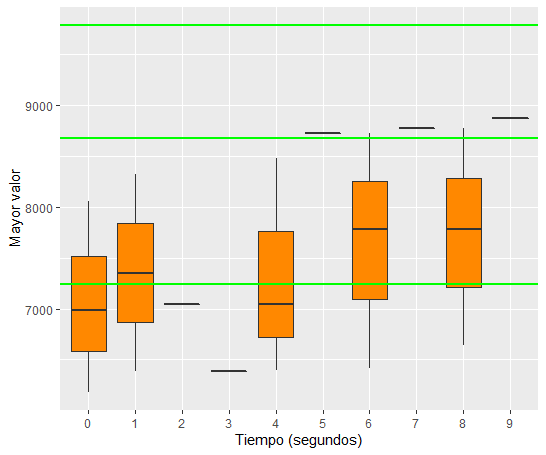
\includegraphics[width=87mm]{FiguraR3C1P0.1.png}}
\subfigure[Probabilidad de mutación = 0.3]{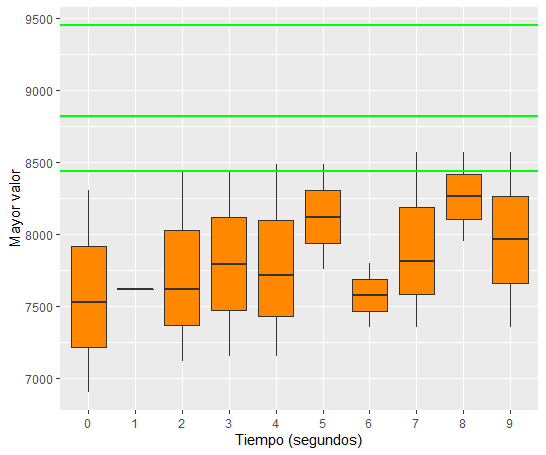
\includegraphics[width=87mm]{FiguraR3C1P0.3.png}}
\subfigure[Probabilidad de mutación = 0.6]{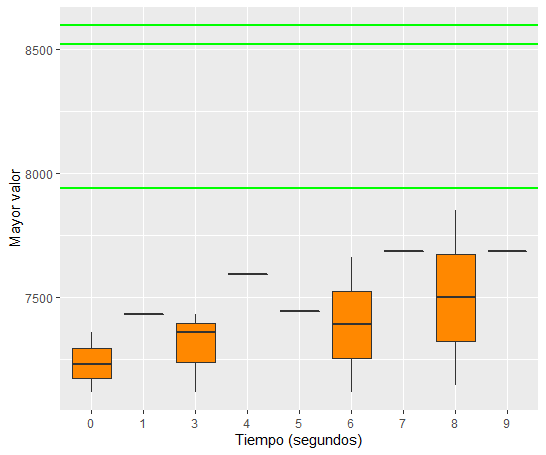
\includegraphics[width=87mm]{FiguraR3C1P0.6.png}}
\caption{Mayor valor para cada tiempo de acuerdo a cada probabilidad de mutación para el código 1 de la regla 3.} 
\label{f7}
\end{figure}

\begin{table}[h!]
\centering
\caption{Resultados de la prueba estadística.}
\smallskip

\begin{tabular}{ |p{4cm}|p{8cm}|}
 \hline
 Outliers & $0$ \\
 \hline
 Normalidad por grupo & $0.1$: $p$ = $0.0143$ / $0.3$: $p$ = $0.0395$ / $0.6$: $p$ = $0.2080$ \\
 \hline
 Kruskal Wallis & $p$ = $0.2004$ \\
 \hline
\end{tabular}
\label{Cuadro13}
\end{table}

\begin{table}[h!]
\centering
\caption{Resultados al aplicar la prueba \texttt{Wilcoxon}.}
\smallskip

\begin{tabular}{|p{1.7cm}|p{1.7cm}|p{1.7cm}|}
 \hline
Valor de $p$ & $0.1$ & $0.3$ \\
 \hline
 $0.3$ & $0.990$ & -   \\
 \hline
 $0.6$ & $0.990$ & $0.087$  \\
 \hline
\end{tabular}
\label{Cuadro14}
\end{table}

Hipótesis nula : Las medias son iguales en todos los grupos. Se acepta esta hipótesis.

\newpage
\begin{figure}[h!]
\centering
\subfigure[Cruzamientos = 10]{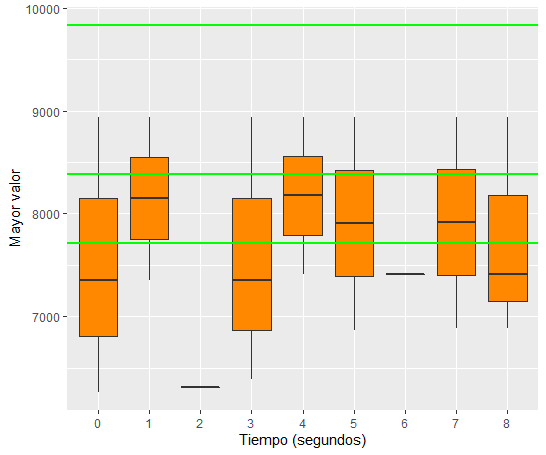
\includegraphics[width=87mm]{FiguraR3C2R10.png}}
\subfigure[Cruzamientos = 15]{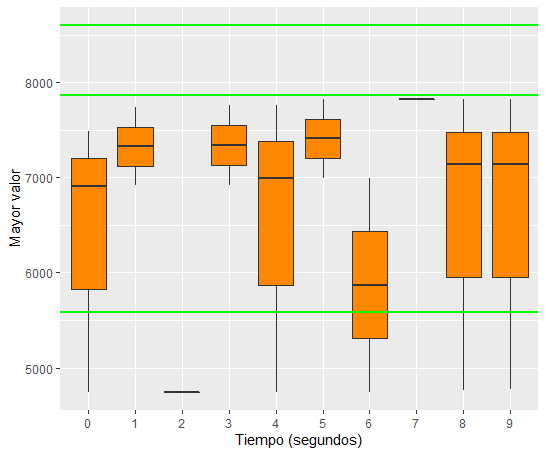
\includegraphics[width=87mm]{FiguraR3C2R15.png}}
\subfigure[Cruzamientos = 20]{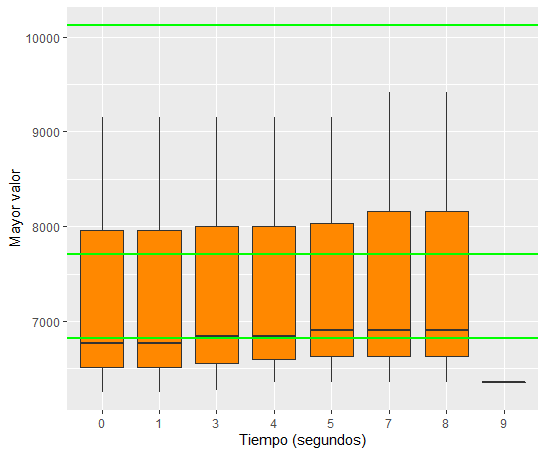
\includegraphics[width=87mm]{FiguraR3C2R20.png}}
\caption{Mayor valor para cada tiempo de acuerdo a cada cantidad de cruzamientos para el código 2 de la regla 3.} 
\label{f8}
\end{figure}

\begin{table}[h!]
\centering
\caption{Resultados de la prueba estadística.}
\smallskip

\begin{tabular}{ |p{4cm}|p{8cm}|}
 \hline
 Outliers & $0$ \\
 \hline
 Normalidad por grupo & $10$: $p$ = $00.00258$ / $15$: $p$ = $0.00010$ / $20$: $p$ = $0.00005$ \\
 \hline
 Kruskal Wallis & $p$ = $0.3074$ \\
 \hline
\end{tabular}
\label{Cuadro15}
\end{table}

\begin{table}[h!]
\centering
\caption{Resultados al aplicar la prueba \texttt{Wilcoxon}.}
\smallskip

\begin{tabular}{|p{1.7cm}|p{1.7cm}|p{1.7cm}|}
 \hline
Valor de $p$ & $10$ & $15$ \\
 \hline
 $15$ & $0.27$ & -   \\
 \hline
 $20$ & $0.73$ & $0.92$  \\
 \hline
\end{tabular}
\label{Cuadro16}
\end{table}

Hipótesis nula : Las medias son iguales en todos los grupos. Se acepta esta hipótesis.

\newpage
\begin{figure}[h!]
\centering
\subfigure[Población = 25]{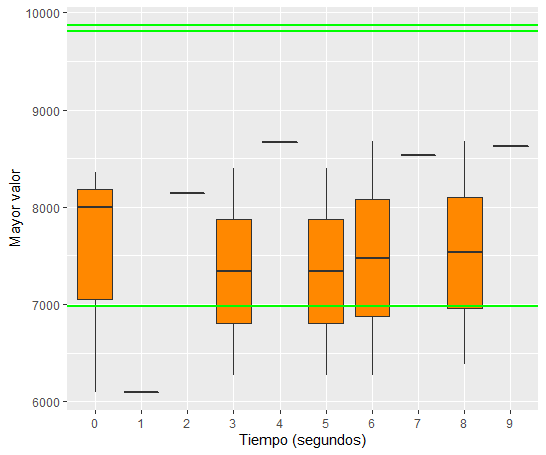
\includegraphics[width=87mm]{FiguraR3C3S25.png}}
\subfigure[Población = 35]{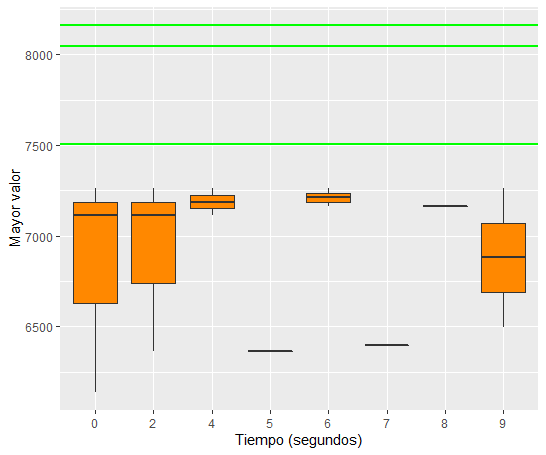
\includegraphics[width=87mm]{FiguraR3C3S35.png}}
\subfigure[Población = 45]{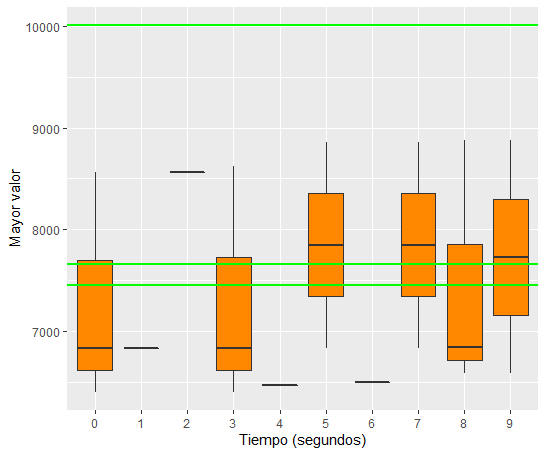
\includegraphics[width=87mm]{FiguraR3C3S45.png}}
\caption{Mayor valor para cada tiempo de acuerdo a cada tamaño de población para el código 3 de la regla 3.} 
\label{f9}
\end{figure}

\begin{table}[h!]
\centering
\caption{Resultados de la prueba estadística.}
\smallskip

\begin{tabular}{ |p{4cm}|p{8cm}|}
 \hline
 Outliers & $0$ \\
 \hline
 Normalidad por grupo & $25$: $p$ = $0.00063$ / $35$: $p$ = $0.00103$ / $45$: $p$ = $0.00020$ \\
 \hline
 Kruskal Wallis & $p$ = $0.5021$ \\
 \hline
\end{tabular}
\label{Cuadro17}
\end{table}

\begin{table}[h!]
\centering
\caption{Resultados al aplicar la prueba \texttt{Wilcoxon}.}
\smallskip

\begin{tabular}{|p{1.7cm}|p{1.7cm}|p{1.7cm}|}
 \hline
Valor de $p$ & $25$ & $35$ \\
 \hline
 $35$ & $0.48$ & -   \\
 \hline
 $40$ & $1$ & $1$  \\
 \hline
\end{tabular}
\label{Cuadro18}
\end{table}

Hipótesis nula : Las medias son iguales en todos los grupos. Se acepta esta hipótesis.
\newpage

A continuación se muestra el código utilizado para realizar los diagramas caja-bigote y las prueba estadística \texttt{Kruskal Wallis} para el código 1 de la regla 1, este código también se aplica a las demás reglas únicamente cambiando los respectivos valores que se ocupan analizar:

\lstset{style=mystyle}
\begin{lstlisting}[language=R, caption= Código para las pruebas estadísticas \texttt{Kruskal Wallis} y \texttt{Wilcoxon}.]
library(ggplot2)
df$Segundo = as.factor(df$Segundo)
dfs = split.data.frame(df, f = df$Mutacion)

ggplot(dfs$`0.1`, aes(x= Segundo, y= Mejor)) + 
  geom_boxplot(fill = "#F8766D")+
  labs(x = "Tiempo (segundos)", y = "Mayor valor", title = 'pm = 0.1')+
  geom_hline(aes(yintercept=Optimo), colour="green", size= 1)

ggplot(dfs$`0.3`, aes(x= Segundo, y= Mejor)) + 
  geom_boxplot(fill = "#F8766D")+
  labs(x = "Tiempo (segundos)", y = "Mayor valor", title = 'pm = 0.3')+
  geom_hline(aes(yintercept=Optimo), colour="green", size= 1)

ggplot(dfs$`0.6`, aes(x= Segundo, y= Mejor)) + 
  geom_boxplot(fill = "#F8766D")+
  labs(x = "Tiempo (segundos)", y = "Mayor valor", title = 'pm = 0.6')+
  geom_hline(aes(yintercept=Optimo), colour="green", size= 1)

library(tidyverse)
library(ggpubr)
library(car)
library(rstatix)
library(rapportools)
library(readr)
library(gridExtra)

#PRUEBA ESTADISTICA...
#Estadisticas descriptivas
df %>%
  group_by(Mutacion) %>%
  get_summary_stats(Mejor, type = "mean_sd")

#SUPUESTOS PARA ANOVA
#1:Outliers
df %>%
  group_by(Mutacion) %>%
  identify_outliers(Mejor)

#2:Normalidad por Shapiro
df %>%
  group_by(Mutacion) %>%
  shapiro_test(Mejor)

#3:Homogeneidad de varianza con prueba Levene
df %>%
  levene_test(Mejor~Mutacion)

#PRUEBA ESTADISTICA KRUSKAL WALLIS
kruskal.test(Mejor ~ Mutacion, data = df)

#PRUEBA WILCOXON
pairwise.wilcox.test(df$Mejor, df$Mutacion)
\end{lstlisting}

\newpage
\section{Conclusi\'{o}n}
Con base en los diagramas caja-bigote obtenidos puedo concluir que en la regla 1 conforme pasan los segundos se logra alcanzar el valor óptimo en probabilidades de mutación más grandes, lo mismo sucede con la variación de los cruzamientos, también se logra alcanzar el valor óptimo conforme pasan los segundos y con respecto a la variación del tamaño de población éste no tiene tanta influencia en la posibilidad de alcanzar el valor óptimo. Para la regla 2 de igual manera conforme avanzan los $10$ segundos se puede llegar al valor óptimo sobre todo con probabilidades de mutación grandes y en cuando a los cruzamientos también se observa este comportamiento, solamente en el tamaño de población no se tiene una relación entre el tiempo y los valores mayores obtenidos. En la regla 3 se puede observar un comportamiento diferente, en la mayoría de las combinaciones desde el segundo $1$ se logra alcanzar el valor óptimo y este comportamiento se mantiene. 
\smallskip

En general ésta práctica se me dificultó la parte estadística pero con el apoyo de mis compañeros finalmente pude realizarla.
\newpage

\bibliography{referencias}
\bibliographystyle{plainnat}

\end{document}